\chapter{Các Bài toán Đệ quy}\label{ch:recurrent-problems}

Ở chương này, chúng ta sẽ khám phá ba bài toán ví dụ.
Chúng có hai điểm chung:
đều đã được nghiên cứu rất kĩ bởi các nhà toán học;
và lời giải của chúng đều sử dụng ý tưởng \textit{đệ quy}, tức là lời giải cho mỗi bài toán phụ thuộc vào lời giải các bài toán con nhỏ hơn của bài toán đó.

\section{Bài toán Tháp Hà Nội}

\marginpar[Giơ tay lên nếu đây là lần đầu bạn nghe về bài toán này. Ok, số còn lại có thể lướt đến \eqref{eq:1.1}]{Giơ tay nếu đây là lần đầu bạn nghe về bài toán này. Ok, số còn lại có thể lướt đến \eqref{eq:1.1}}

Chúng ta sẽ xem xét một câu đố thú vị, tên là Bài toán Tháp Hà Nội, được phát minh bởi nhà toán học người Pháp Edouard Lucas năm $1883$.
Chúng ta có một tháp gồm tám đĩa, được xếp theo thứ tự kích thước giảm dần trên một trong ba cột.

\begin{center}
    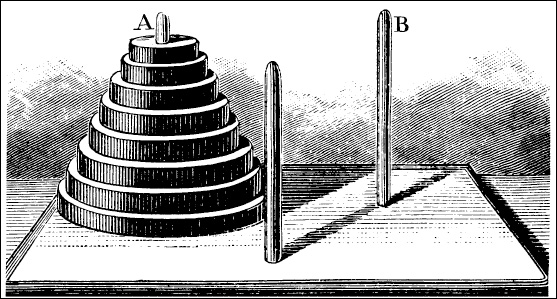
\includegraphics[width=.5\textwidth]{assets/chapter1/Tower of Hanoi}
\end{center}

Mục tiêu của chúng ta, là di chuyển hết tòa tháp sang một trong các cột còn lại, trong đó mỗi lượt chỉ được di chuyển một đĩa từ cột này sang cột khác, và đĩa lớn không bao giờ được đặt trên đĩa nhỏ hơn.

\marginpar[Làm bằng vàng cơ à. Sao không phải bê tông?]{Làm bằng vàng cơ à. Sao không phải bê tông?}

Lucas còn viết một huyền thoại về tòa Tháp Brahma khổng lồ, với 64 đĩa làm bằng vàng nguyên chất và ba cột làm từ kim cương.
Ông kể rằng, ngày mà thời gian bắt đầu trôi, Đấng Sáng Thế đã đặt những chiếc đĩa vàng này trên cột thứ nhất, rồi lệnh cho những nhà sư phải chuyển hết số đĩa sang cột thứ ba, theo quy tắc như trên.
Họ làm việc vất vả xuyên cả ngày đêm.
Khoảnh khắc họ đặt chiếc đĩa cuối cùng xuống, tòa Tháp sẽ sụp đổ, và thế giới sẽ đi đến hồi kết.

\begin{equation}\label{eq:1.1}
    \begin{aligned}
        & \mathsf{T}_0 = 0; \\
        & \mathsf{T}_n = 2 \mathsf{T}_{n - 1} + 1, \text{ với } n > 0.
    \end{aligned}
\end{equation}